\chapter{REMAINING TASKS}
 
The core software pipeline described is completed and has
been validated algorithmically. The remaining work falls into
four categories: hardware-dependent data collection, quantitative
evaluation against the metrics defined in the proposal, robustness
testing, and final documentation.
 
\section{Hardware Calibration and Live Capture}
 
\begin{itemize}
    \item \textbf{Improve extrinsic calibration accuracy} (currently
    2.43--3.63\,px, above the $\sim$1.0\,px target): capture more
    checkerboard shots specifically within the shared 3-camera overlap
    zone, with wider pose variety, since this is the most likely source
    of the elevated error and the outlier reconstructions.
    \item Re-run \texttt{main.py} after re-calibration and confirm the
    12.76\% implausible-reconstruction rate decreases.
    \item Complete intrinsic calibration re-checks only if a camera's
    lens/zoom/focus changes  current intrinsic results (0.21--0.31\,px)
    are already solid and do not need rework.
    \item \textbf{Re-measure FPS} after the inference-downscaling and
    thread-pool fixes, using\texttt{analyze\_dataset.py} on a fresh session.
    \item \textbf{Investigate the outlier reconstruction rate}: re-run
    with \texttt{MIN\_CONFIDENCE\_TO\_USE\_VIEW} raised from 0.3 to 0.6 in
    \texttt{config.py}, and compare the outlier percentage
    (\texttt{analyze\_dataset.py}) before and after.
\end{itemize}
 
\section{Quantitative Evaluation}
 
The following metrics, specified in the proposal, still require live data
collection to report:
 
\begin{itemize}
    \item \textbf{Landmark detection performance}: precision, recall,
    F1-score for MediaPipe Pose/Hands against manually verified ground
    truth poses.
    \item \textbf{3D reconstruction accuracy}:  mean reconstruction error
    against known reference measurements or fixed calibration poses. Unlike the synthetic validation in Chapter 6, this must use
    real camera noise and real calibration error.
    \item \textbf{Real-time processing performance}: FPS, average
    per-frame processing time, CPU utilization.
    \item \textbf{Simulation replication latency}: delay between capture
    timestamp and simulation update.
    \item \textbf{Dataset completeness}: percentage of frames with valid
    joint data across a full recording session.
\end{itemize}
 
\section{Occlusion Robustness Testing}
 
Controlled occlusion experiments : manually
blocking one camera's view during capture and measuring the resulting
change in landmark detection continuity, reconstruction accuracy, and
simulation stability, to verify the multi-camera redundancy behaves as
intended when a view is lost.

\section{Remaining Milestones}
\begin{figure}[ht]
    \centering
    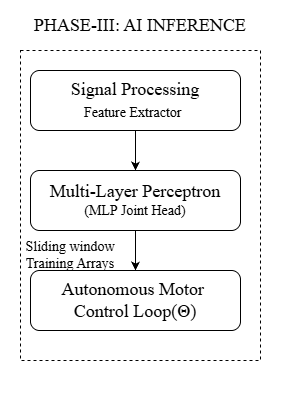
\includegraphics[width=0.4\textwidth]{src/images/PhaseIII.png}
    \caption{System block Diagram Phase III}
    \label{phaseIII}
\end{figure}

\begin{enumerate}
    \item \textbf{Filter Optimization and Validation}  
          Perform parameter sweep on $f_{\text{min}}$ and $\beta$ and evaluate 
          trajectory smoothness using quantitative metrics.
    
    \item \textbf{Structured Dataset Collection}  
          Capture a diverse set of motion sequences for stabilization analysis 
          and LSTM training.
    
    \item \textbf{Trajectory Stability Evaluation}  
          Measure jitter, variance, and acceleration before and after filtering.
    
    \item \textbf{LSTM Model Training and Testing}  
          Implement stacked LSTM refinement and validate performance on 
          held-out sequences.
    
    \item \textbf{Comparative Benchmarking and Reporting}  
          Produce tables, graphs, and discussion comparing system performance 
          across all refinement stages.
\end{enumerate}

\section{Risks and Mitigation Strategies}

\subsection*{Risk 1: Insufficient Dataset Stabilization}

Current dataset capture lacks systematic evaluation of jitter and 
trajectory consistency.

\textbf{Mitigation:}  
Define objective metrics (RMSE, coordinate variance, maximum acceleration) 
and conduct controlled evaluation experiments.

\subsection*{Risk 2: One Euro Filter Parameter Sensitivity}

Improper parameter selection may lead to over-smoothing or residual jitter.

\textbf{Mitigation:}  
Conduct structured parameter tuning and document results empirically.

\subsection*{Risk 3: LSTM Training Ineffectiveness}

The LSTM refinement stage may not significantly outperform the analytical filter.

\textbf{Mitigation:}  
Use simplified architecture, regularization, and sufficient motion diversity 
to improve generalization performance.

\subsection*{Risk 4: Timeline Compression}

Remaining tasks involve experimentation and benchmarking, which may require 
additional iteration time.

\textbf{Mitigation:}  
Prioritize filter validation and dataset stabilization first, ensuring 
a stable analytical baseline before implementing learning-based refinement.

\section{Overall Assessment}

The project has successfully established its structural foundation, including 
calibration, triangulation, and preliminary robotic simulation. The remaining 
work focuses primarily on stabilization, evaluation, and refinement rather 
than architectural redesign. With systematic experimentation and parameter 
optimization, the system can be matured into a fully validated motion capture 
and dataset generation framework within the remaining timeline.